
\label{ch:Design}

Dans ce chapitre, nous allons implémenter, dans le langage du logiciel Max, les formules mathématiques présentées précédemment. De plus, nous allons introduire d'autres effets spectraux et des variations dans le contexte du vocodeur de phase.

Par ailleurs, nous allons presenter les objets Max qui encapsulent\footnote{Encapsuler : créer un sub-patch qui contient un ensemble d'objets / fonctions } des fonctions mathématiques telles que FFT, IFFT et d’autres transformations. On peut attendre de ce partie qu'il permet de comprendre la plupart des outils spectraux que Max offre à l’utilisateur. Parallèlement, on va construire une série d’outils efficaces pour structurer un simple vocodeur de phase.

\section{Objets Max}

Dans cette section, nous allons mentionner quelques-uns des objets spectraux de base de Max fournis directement par la librairie standard, et nous analyserons leurs fonctionnalités.

Dans Max, il existe 3 catégories d’objets :
\begin{enumerate}
    \item
    Les objets logiques utilisés pour les expressions et les calculs logiques; 
    \item
    Les objets signaux, pour le traitement du signal, suivis généralement par une indication \guillemotleft$ \thicksim $\guillemotright après leur nom ; 
    \item
    Les objets Jitter qui sont utilisés pour les données multidimensionnelles, tels que images, formes 3D, etc.
\end{enumerate}

La manière dont un objet spectral fonctionne dans Max est quelque peu différente de celle des autres objets signaux. Ils sont déployés dans un environnement spécial appelé \textit{PFFT}$\thicksim $. Le PFFT contient, fréquemment, une FFT et une IFFT. La majorité des objets dans le PFFT traitent des données bidimensionnelles, par conséquent, ils sont traités dans un patch différent.

\subsubsection{FFT$\thicksim$}
    L'objet $ \textit{fft}\thicksim $ appartient à la famille de signaux, comme le précise l'indicateur $ \thicksim $. C'est l'objet qui effectue la transformation rapide de Fourier. Il y a deux entrées correspondantes aux parties réelle et imaginaire. Ordinairement, on utilise l'entrée réelle afin de effectuer une FFT a un signal. Il y a trois sorties a l'objet, une pour la partie réelle de l'exponentielle complexe, une pour la partie imaginaire et un compteur qui garde l’index des harmoniques de la transformation de Fourier.

    Dans la transformation de Fourier fenêtrée habituelle:
    \begin{equation}
        X_k = \sum_{n=0}^{N-1} x_n \; e^{-j \frac{2 \pi k n}{N}}
    \end{equation}

    Où k est l’indice de l'harmonique et les coordonnées complexes correspondantes sont $ \sum_{n = 0}^k x_n + cos (2 \pi t) $ pour la partie réelle et $ \sum_{n = 0}^k x_n + j sin (2 \pi t) $ pour l’imaginaire. Bien entendu, la réduction correspondante de la ramification calculée est appliquée par l’algorithme FFT présenté au chapitre précédent.

\subsubsection{IFFT$\thicksim$}
    
    De manière similaire, la FFT inverse est traitée par la fonction d'objet appropriée avec les entrées et les sorties inverses.

\subsubsection{cartopol$\thicksim$}
    
    Il n’est généralement pas utile d’utiliser ces coordonnées cartésiennes, produites par le \textit{fft}$\thicksim $ correspondant aux parties réels et imaginaires du plan $ \mathbb {C}^2 $. Par conséquent, un objet transformant les coordonnées cartésiennes en une forme polaire appelée \textit{cartopol}$\thicksim $ est fréquemment déployé. Cet objet a donc deux entrées (réelle et imaginaire) et génère une phase et une magnitude pour chaque index.

\subsubsection{poltocar$\thicksim$}
    
    Exactement la fonction inverse de \textit{cartopol}$\thicksim $. L’objet \textit{poltocar}$\thicksim $ transforme des coordonnées polaires (deux entrées) aux coordonnées Cartésiennes (deux sorties).

\subsubsection{FFTinfo$\thicksim$}
    
    \textit{FFTinfo}$\thicksim $ est très fréquemment utilisé et il fournit des informations sur les paramètres de la FFT, tels que la taille de la fenêtre, etc.

\subsubsection{\textit{framedelta}$\thicksim$}
    
    \textit{framedelta}$\thicksim$ est un objet très important car il calcule la dérivation de phase entre des images successives de la FFT. Également l'objet \textit{phaseaccum}$\thicksim$ peut etre utilisé à la place de \textit{framedelta}$\thicksim$. \textit{phaseaccum}$\thicksim$ qui calcule directement la phase après la derivation.

\subsubsection{gen$\thicksim$}
    
    \textit{gen}$\thicksim$ est un objet qui permet de créer une nouvelle fenêtre speciale d’un patch. Dans cette fenêtre, l'utilisateur peut utiliser un nouvel ensemble de fonctions spécialisées sur le traitement d'un seul échantillon. Les fonctions sont relativement plus simples que l'environnement de codage habituel, mais on peut effectuer un travail plus précis sur les détails. L’environment \textit{gen}$ \thicksim $ est fréquemment utilisé pour effectuer un délai à l'échelle d'échantillons en créant un filtre passe-bas ou des effets similaires.

\section{Détection du pitch}\footnote{Pitch signifie un terme équivalent à la hauteur ou bien à la fréquence}

En utilisant certains de ces objets spectraux Max, nous allons commencer par construire un simple patch afin de trouver la hauteur de la fréquence dominante:

     \begin{displayquote}
         \guillemotleft Les méthodes de détection du pitch dans le domaine fréquentiel dissèquent le signal d'entrée en fréquences constituant le spectre global. Le spectre montre la force des différentes composantes des fréquences contenues dans le signal. Le but est d’isoler la fréquence dominante, ou "pitch", hors du spectre \guillemotright. \footnote{Curtis Roads, \textit{A tutorial in musical signal processing}, 1996. [p. 513], \nocite{Roads1996}}
     \end{displayquote}

De même, nous avons implémenté un patch Max pour trouver la fréquence dominante de la fenêtre FFT. Le patch peut être trouvé dans la figure \ref{PitchTracking}.

    \begin{figure}
        \centering
        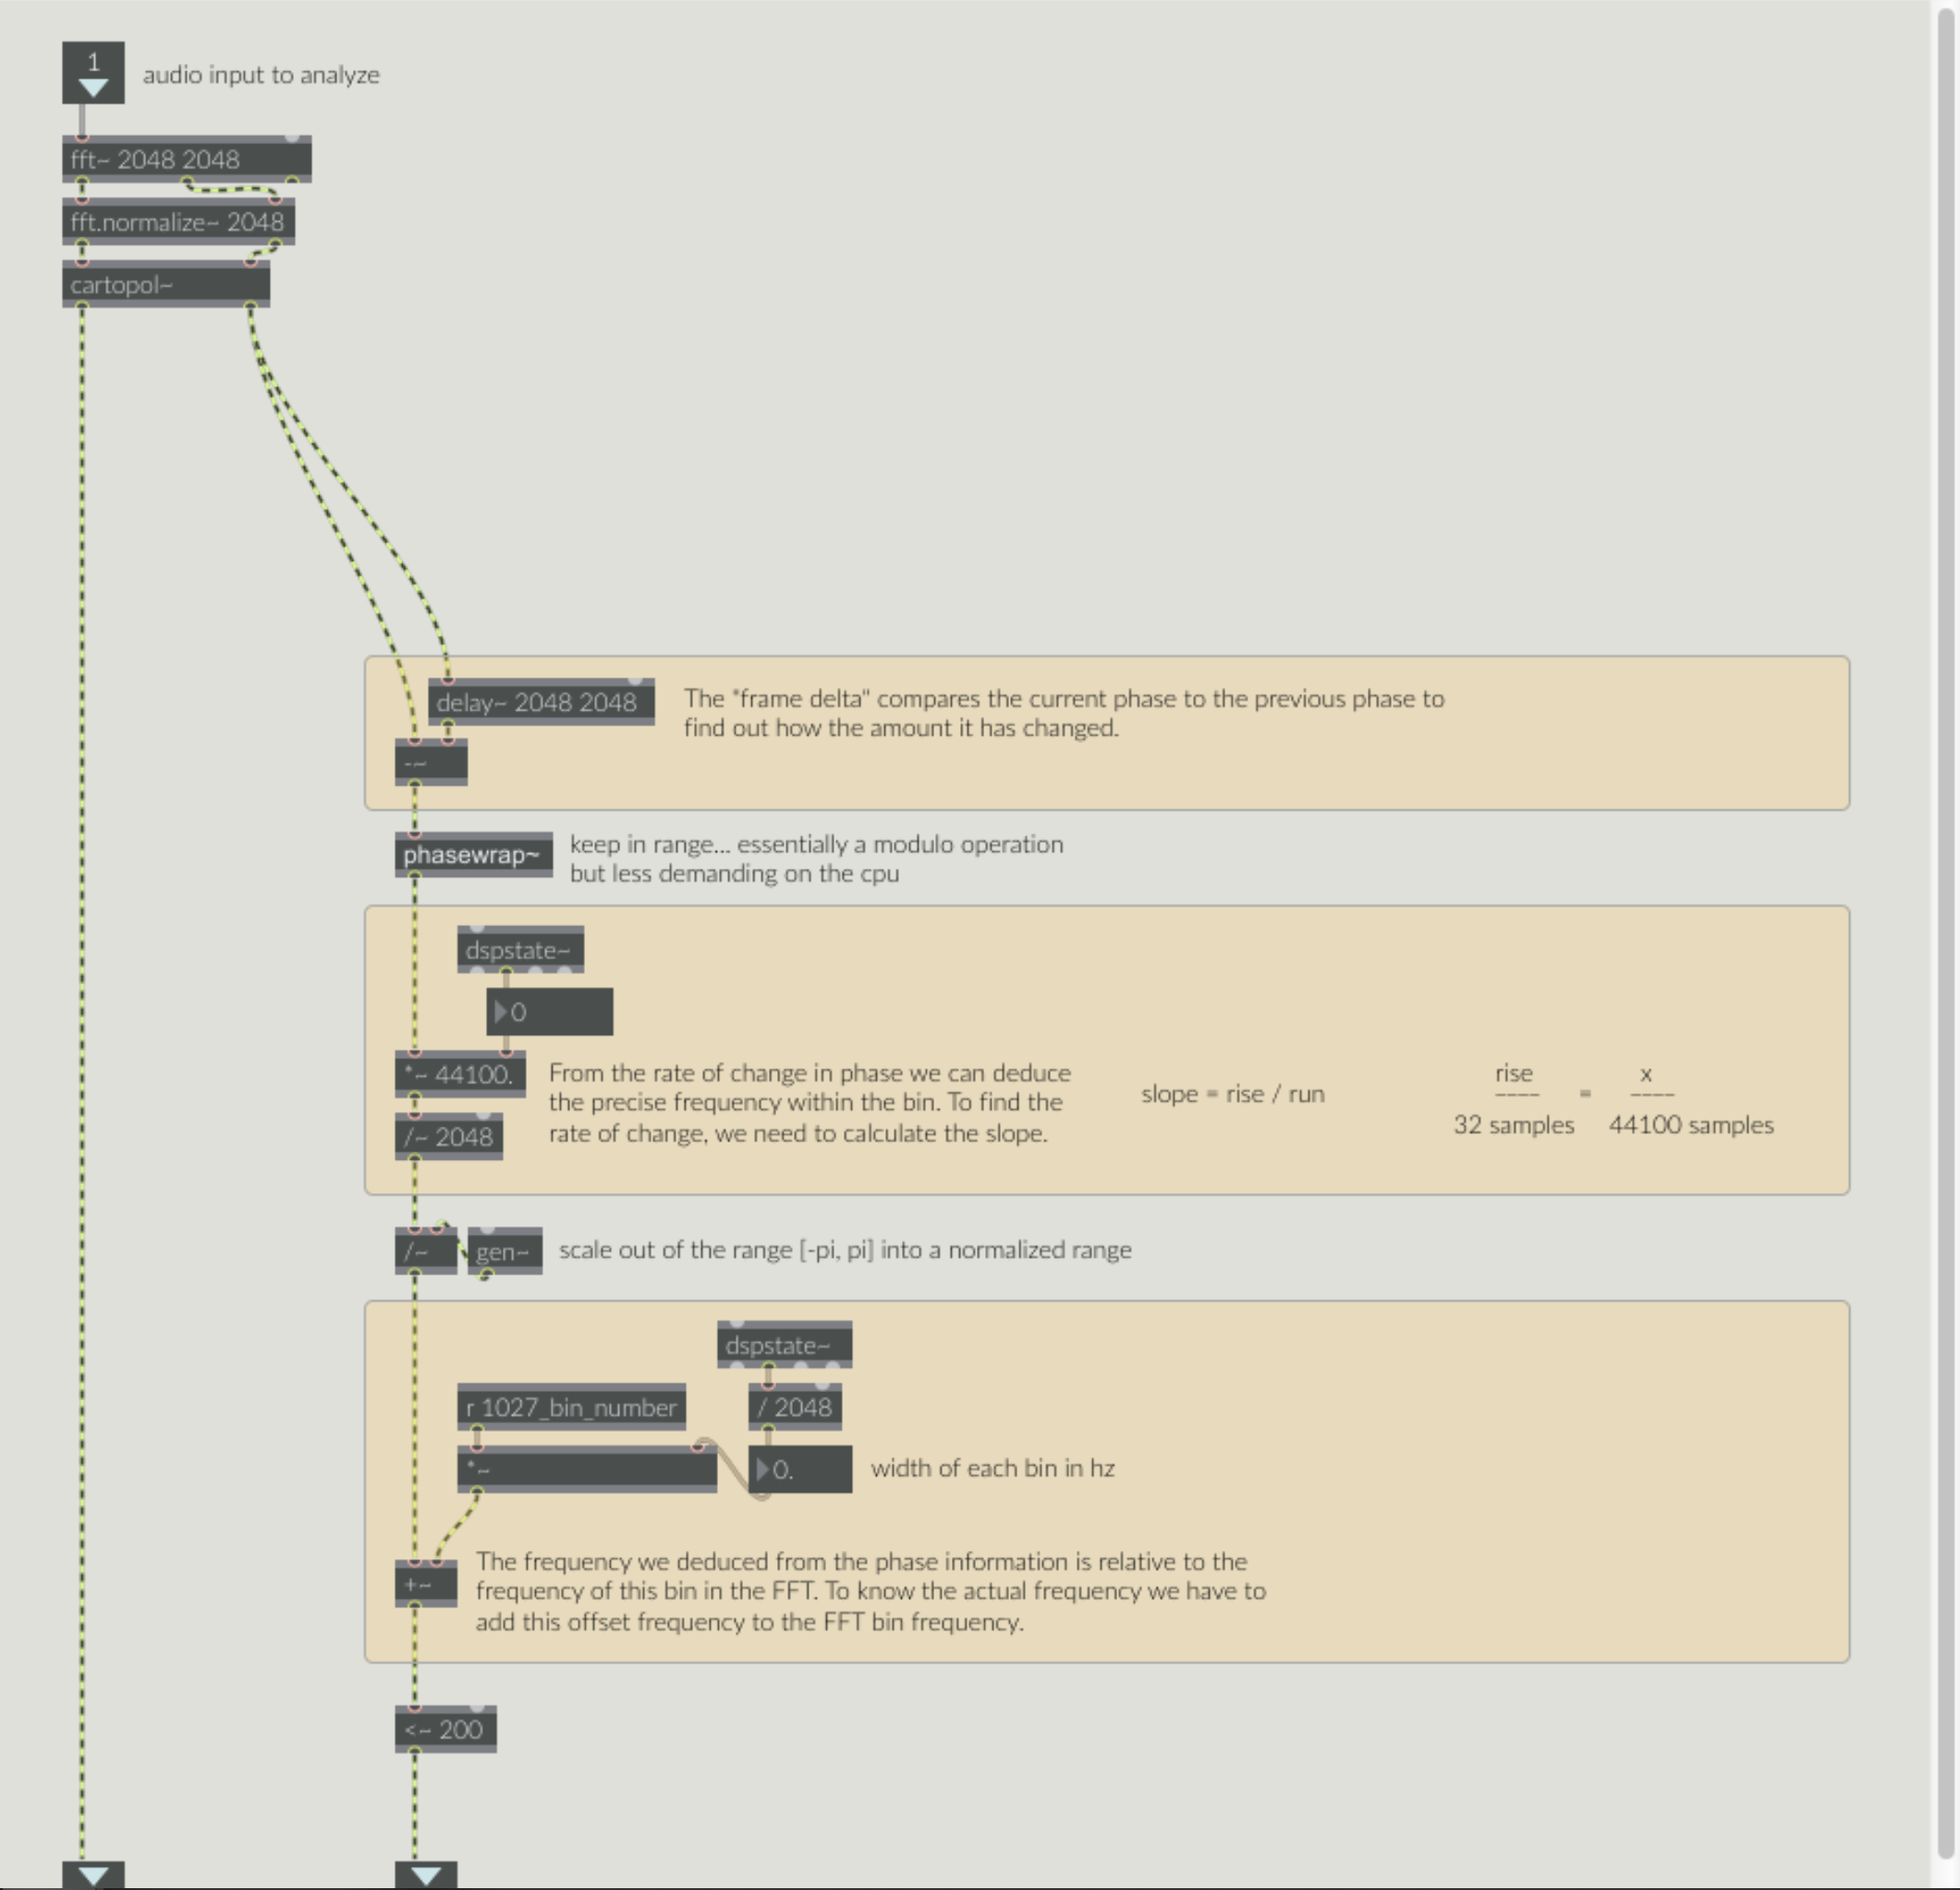
\includegraphics[width = 0.7 \textwidth ]{Graphs/fftTrack.png}
        \caption{Pitch Tracking}
        \label{PitchTracking}
    \end{figure}

Bien entendu, nous utilisons l'objet  \textit{fftin}$\thicksim $ pour transformer le son d’entré dans le domaine fréquentiel. Dans la FFT, nous devons déclarer deux choses. Tout d'abord, le nombre d'images faisant l'objet d'une opposition à la FFT et, deuxièmement, la taille de la fenêtre. Nous rappelons que les deux premières sorties donnent respectivement les composantes réelles et imaginaires. La troisième sortie donne l'harmonique de la fréquence indexée prenant les valeurs correspondantes de $ 0 $ à $ N $, où $ N $ est la taille de la fenêtre FFT.

Pour continuer le patch du simple suivi de la hauteur, nous normalisons les composants réels et imaginaires pour restreindre le flux de données entre des limites calculables. De manière plus détaillée, \textit{fft.normalize}$\thicksim $ est un simple Max externe, créé en code $C++$ à l'aide du Max SDK, qui divise le nombre de chaque sortie par la moitié de la taille de la fenêtre.

Ensuite, nous transformons les coordonnées cartésiennes en coordonnées polaires en utilisant \textit{cartopol}$\thicksim $. Le processus est expliqué à la section 2 sous les termes phase et magnitude. Nous ne sommes intéressés que par la phase de chaque bin. En utilisant la phase de chaque bin, nous pouvons calculer la fréquence exacte de chaque harmonique. Nous rappelons que les termes harmonique, bin et fréquence de Fourier sont les mêmes dans ce contexte.

Tout d'abord, nous retardons la phase de chaque bin d'une fenêtre entière pour calculer le montant de sa dérivation. Ensuite, nous soustrayons la phase en cours de chaque bin par la phase correspondante de la fenêtre précédente. Dans la suite, nous utilisons l’objet \textit{phasewrap}$ \thicksim $ pour découper la valeur comprise entre $ - \pi $ et $ \pi $. Il s'agit essentiellement d'une fonction modulo qui permet de conserver les valeurs dans un intégral computable.

À ce stade, nous devons consulter nos paramètres sonores. Un objet dans Max appelé \textit{dspstate}$ \thicksim $ récupère toutes les données nécessaires que nous pouvons trouver dans $ / Options / Audio \, Status $ dans l'application Max. Nous avons seulement besoin de la fréquence d'échantillonnage. Cette valeur est généralement $ 44100 $Hz donc on la stocké par avance et si elle différente nous la changerions automatiquement. Le signal obtenu à partir de \textit{phasewrap}$ \thicksim $ est multiplié par la fréquence d'échantillonnage et par la suite divisé par la taille de la fenêtre. Ces opérations, qui divisent le SR par la taille de la fenêtre, déduisent des partitions pondérées du spectre. La valeur de la soustraction de la fréquence classe la déviation des partitions fréquentielles. Plus précisément, on divise le spectre audible dans des parties isométriques qui sont déterminées par la division du SR par la taille de la fenêtre. Ensuite, nous normalisons en multipliant par $ 2 \pi $ stocké dans un objet \textit{gen}$\thicksim $, pour manipuler la précision sur le nombre $\pi$. Nous trouvons la position de la partition en multipliant la valeur de la division du spectre par l'indice de l’harmonique correspondante et en l'ajoutant à la déviation pour obtenir la fréquence de cette harmonique.

La division du spectre ou la partition est donnée par:
    \begin{equation*}
        x = \frac{SR}{\text{window size}}
    \end{equation*}

Ensuite, la fréquence est simplement: $ index * x + $ la déviation de phase.

Cette procédure génère toutes les fréquences de toutes les bins de la fenêtre FFT.

L'étape suivante consiste à conserver la fréquence avec la magnitude la plus forte. Nous allons utiliser un objet $ gen \thicksim $. Nous déclarons d'abord les entrées. Nous n'avons besoin que de trois variables. La magnitude de chaque bin, l’index de chaque bin et la taille de la fenêtre FFT. Nous déclarons une seule sortie pour le bin dominant de chaque fenêtre. Le patch est montré dans la figure ci-dessous.
        
    \begin{wrapfigure}{r}{0.5\textwidth}
      \vspace{-20pt}
      \begin{center}
        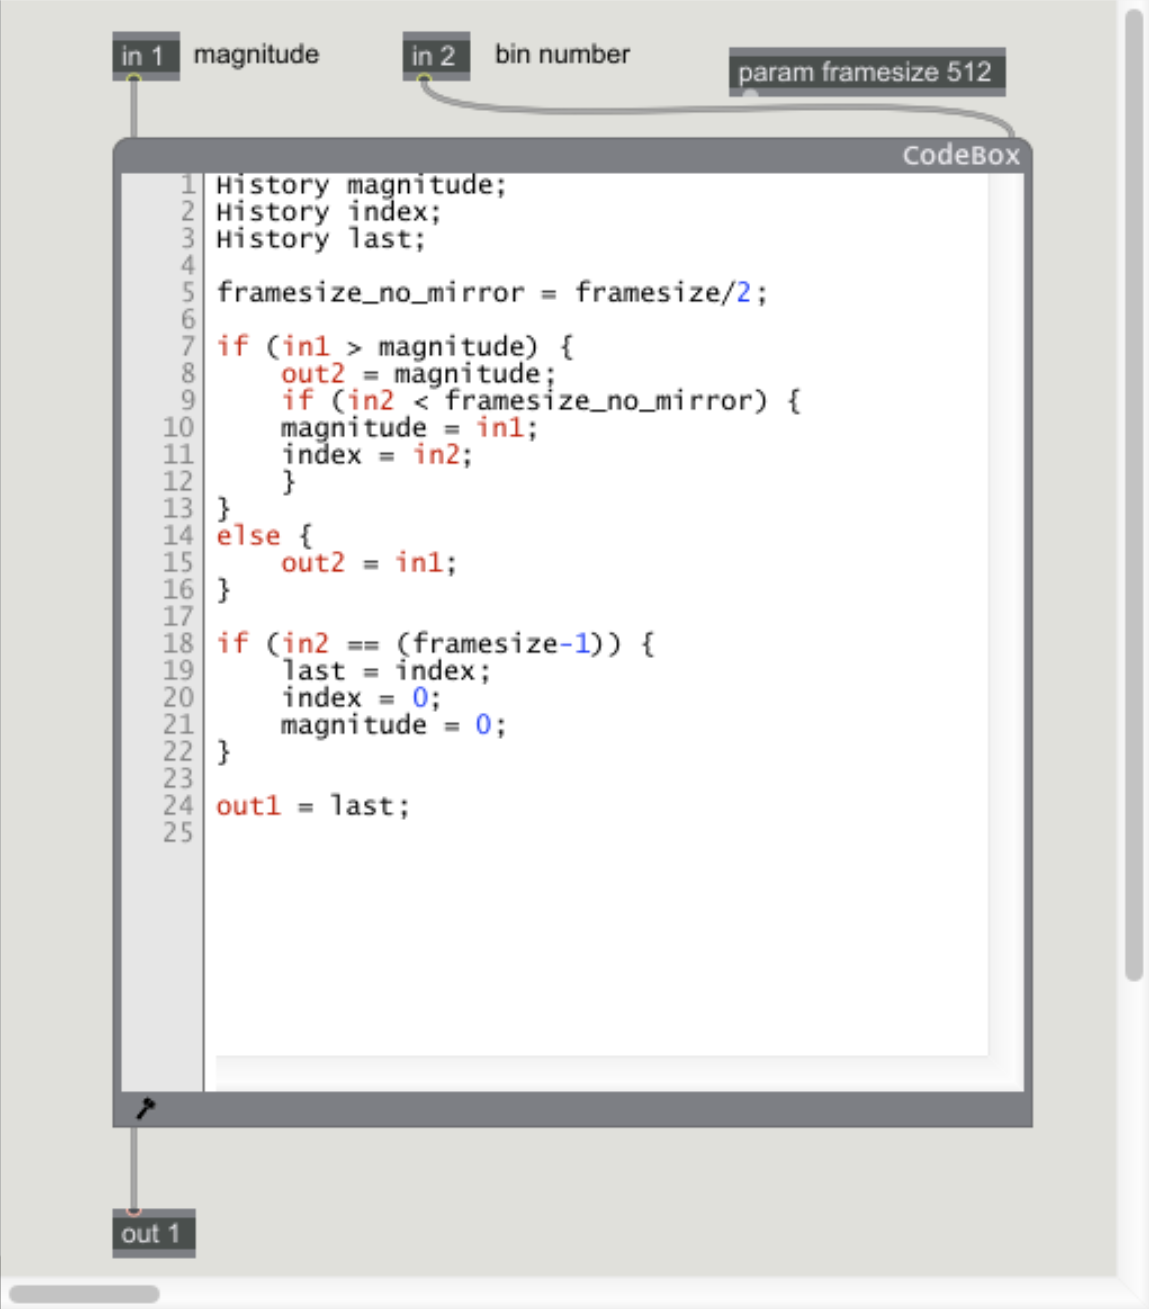
\includegraphics[width=0.48\textwidth]{Graphs/GenfftTrack.png}
      \end{center}
      \vspace{-20pt}
      \caption{Codebox$\thicksim$}
      \vspace{-10pt}
    \end{wrapfigure}

    % \begin{figure}
    %     \centering
    %     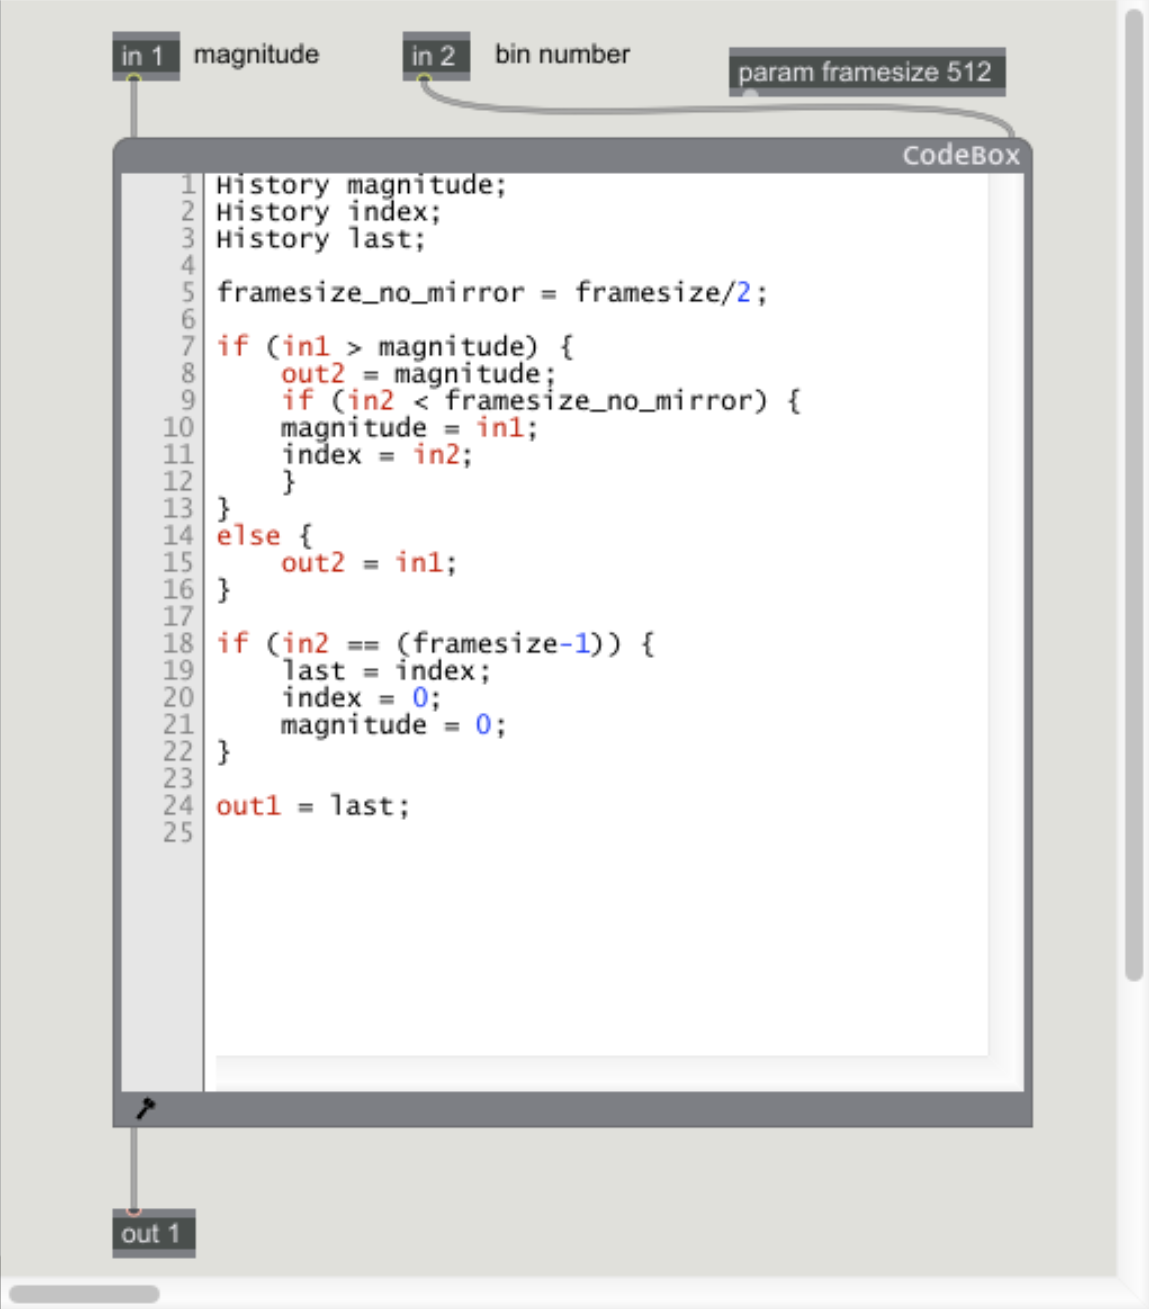
\includegraphics[width = 0.4 \textwidth ]{Graphs/GenfftTrack.png}
    %     \caption{Codebox$\thicksim$}
    %     \label{GenSingle}
    % \end{figure}

Pour calculer le bin le plus fort, nous allons utiliser un objet appelé $ codebox $. $ Codebox $ est un objet qui permet à l'utilisateur de saisir un code sous la forme \guillemotleft traditionnelle \guillemotright. Tout comme le code javascript, nous devons déclarer les variables que nous allons utiliser, qui sont suivant aussi les entrées de cet objet. Les variables dans ce cas sont: magnitude, index, frameSize et last. Où frameSize est la taille de la fenêtre FFT et last est juste une variable qui stocke l'index du bin le plus fort pour la fenêtre précédente.

Le processus de définition du bin le plus fort est mis en œuvre par deux fonctions $if$ imbriquées. Ce processus sera répété pour chaque fenêtre et il déterminera éventuellement les fréquences des cellules les plus puissantes dans toutes les fenêtres. Dans la boucle $if$ imbriquée, nous déterminons si l'index actuel est plus fort que le précédent et nous retournons le résultat. Cela signifie que si la magnitude du $ n-$ième bin est supérieure à celle du ($n-1)-$ième bin, nous stockons sa valeur d'index. La dernière étape consiste à limiter le nombre d'index dans la limite de la taille de la fenêtre afin de terminer la boucle et de réinitialiser les variables.


    \begin{figure}
        \centering
        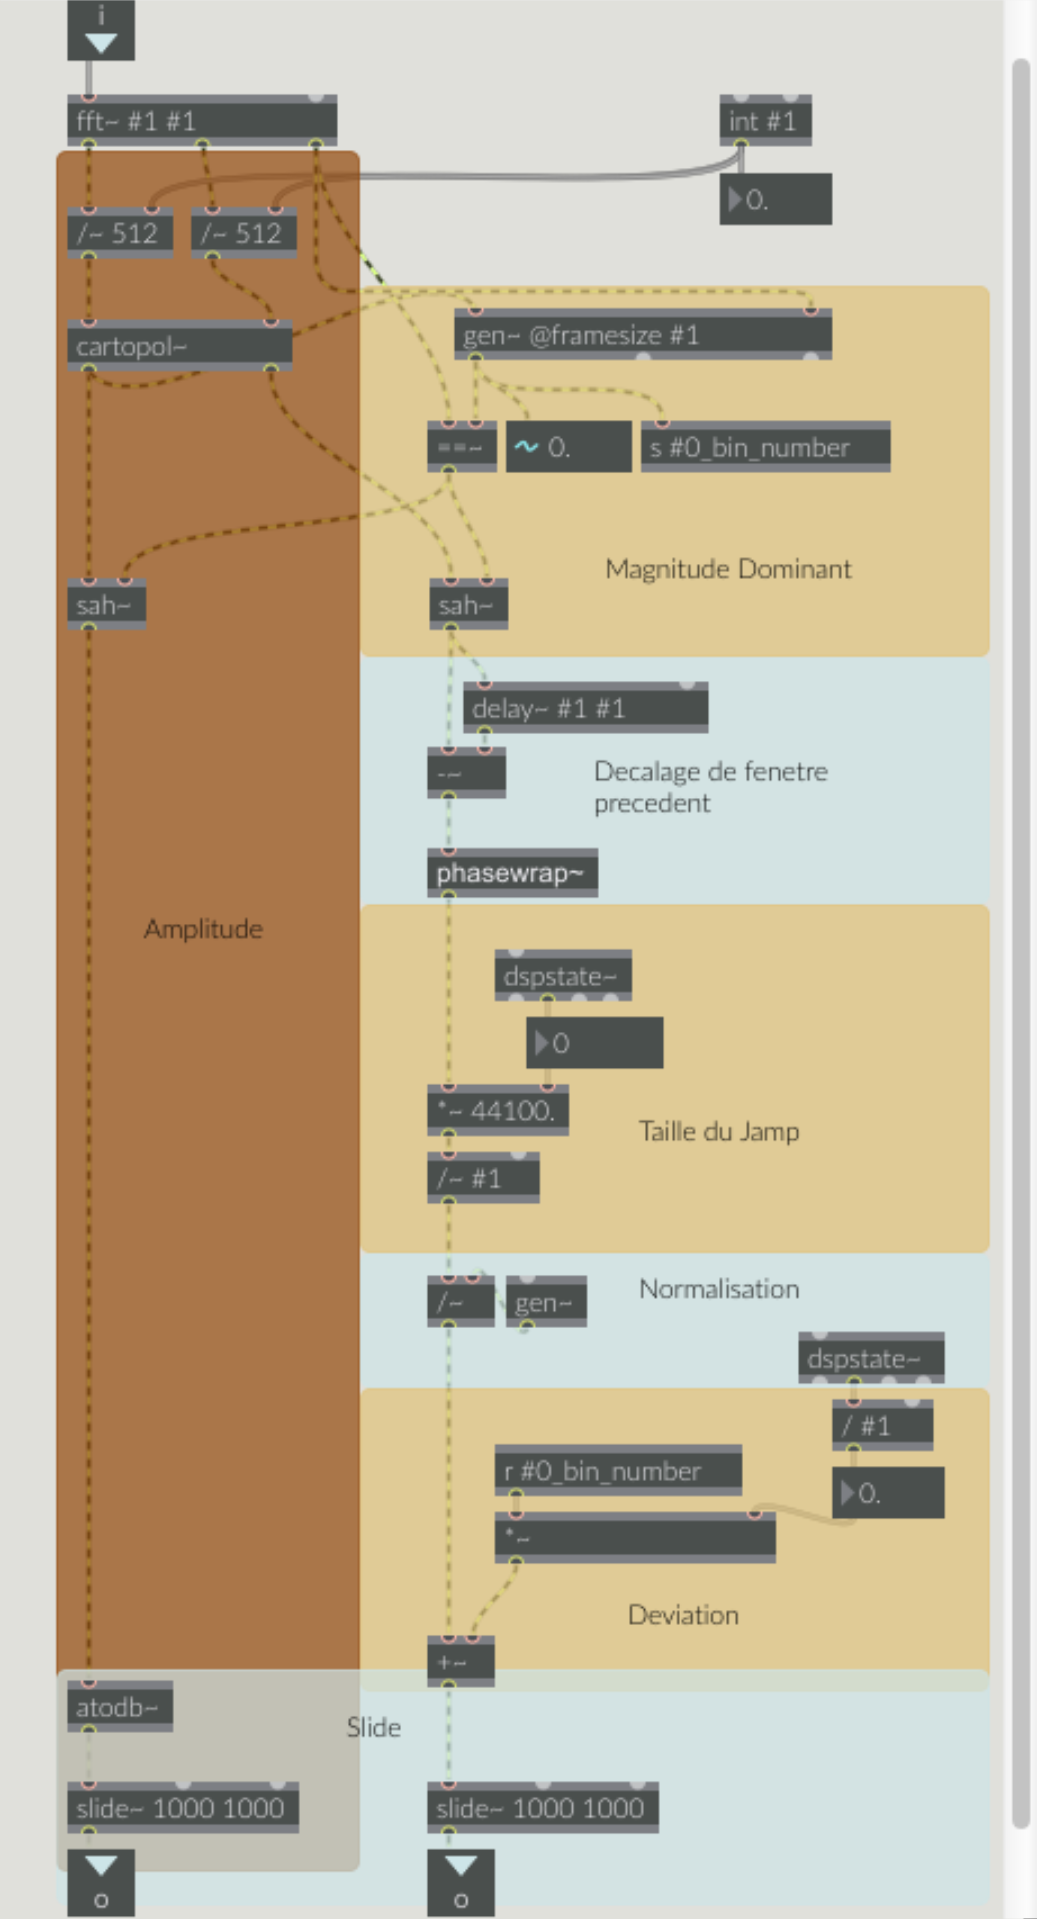
\includegraphics[width = 0.8 \textwidth ]{Graphs/ffttracker.png}
        \caption{Pitch Tracker}
        \label{PitchTracker}
    \end{figure}

Pour localiser l’harmonique le plus fort en précisant la fréquence, quelques fonctions supplémentaires sont nécessaires. La sortie de l'objet \textit{gen}$\thicksim $ est filtrée par un objet \textit{sah}$ \thicksim $. \textit{Sah}$\thicksim $ signifie  \guillemotleft sample holder \guillemotright (stockage d'un échantillon). Avant cela, l'index actuel est comparé à la valeur d'index générée par l'objet \textit{gen}$\thicksim $.  Cette fonction filtre la première entrée de l'objet par un facteur similaire à l'objet \textit{gate}$\thicksim $. Chaque fois que la valeur du facteur change, elle permet à la première entrée d'aller de l'avant et de sortir sa valeur. Nous l'utilisons deux fois, une fois pour la magnitude et une fois pour la phase. De cette façon, seul l’indice de l'harmonique avec la plus grande magnitude va de paire avec la magnitude et la phase correspondante. Nous utilisons le système fourni précédemment pour trouver la fréquence exacte et nous traduisons les coordonnées polaires de l'amplitude en dB. Enfin, nous utilisons un objet \textit{slide}$\thicksim $ pour lisser le résultat. Le patch final est montré dans la figure \ref{PitchTracker}. Cette méthode évite de calculer chaque fois la fréquence si le son est périodique et donc la fréquence dominante ne change pas.

\subsection{Détection des pitchs multiples}

Pour créer un patch de suivi des hauteurs multiples, nous utilisons la méthode du suivi de la hauteur simple unique avec quelques modifications. La majorité des calculs ont lieu dans l'objet $ gen \thicksim $ car l'implémentation de $ codebox $ est copiée en fonction du nombre de hauteurs que l'on souhaite calculer.

    \begin{figure}
        \centering
        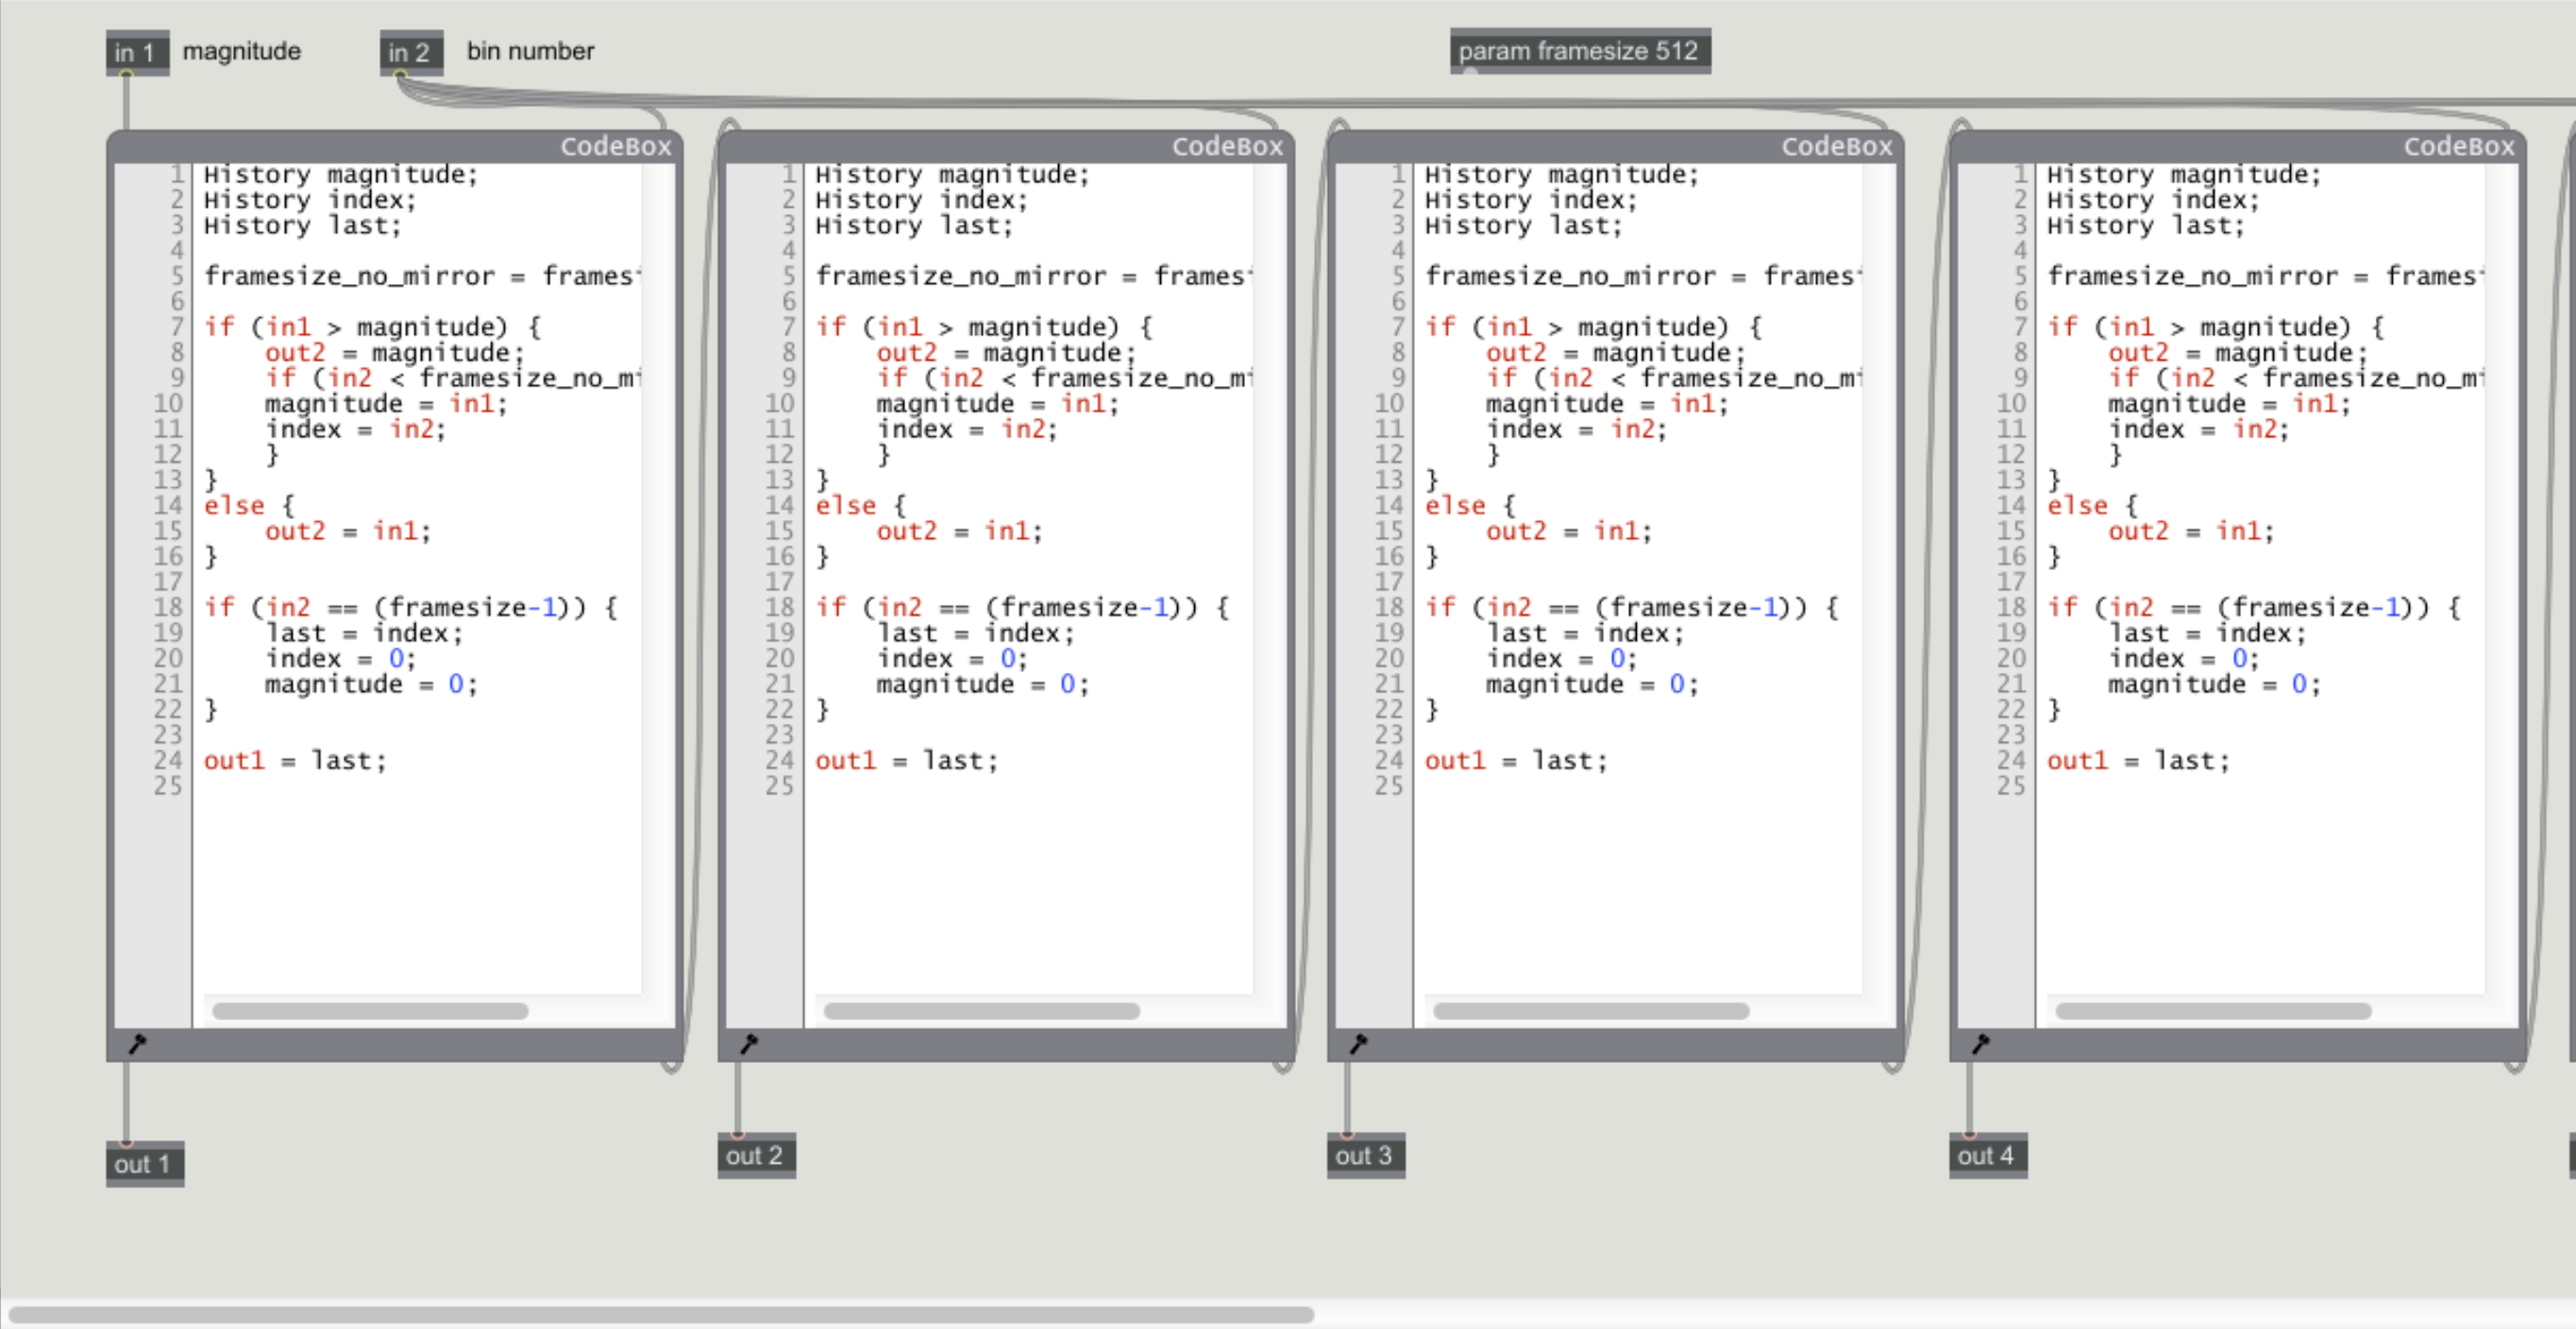
\includegraphics[width = \textwidth]{Graphs/GenMultiple.png}
        \caption{Gen multiple}
        \label{GenMultiple}
    \end{figure}

La figure \ref{GenMultiple} permet de visualiser comment on peut calculer une série des harmoniques les plus fortes de chaque fenêtre. L'objectif est de fournir une quantité suffisante d'informations sur les composantes spectrales de base du son.

Comme le suggère la figure \ref{GenMultiple}, la sortie de chaque \textit{codebox} correspond à l'entrée de la suivante, calculant ainsi le prochain indice le plus fort de la fenêtre. La quantité d’objets \textit{codebox} utilisée correspond au nombre des harmoniques que nous allons afficher.

La mise en œuvre de la méthode de la localisation des plusieurs hauteurs peut être montrée à la figure \ref{Analysis}. Nous reproduisons essentiellement le calcul de fréquence pour chaque indice. Le résultat peut être affiché sous forme de liste ou dans différents sorties. Ensuite, on peut utiliser l’objet \textit{mc.cycle$\thicksim $} dans la version Max8, de simples oscillateurs ou résonateurs dans les autres cas.

    \begin{figure}
        \centering
        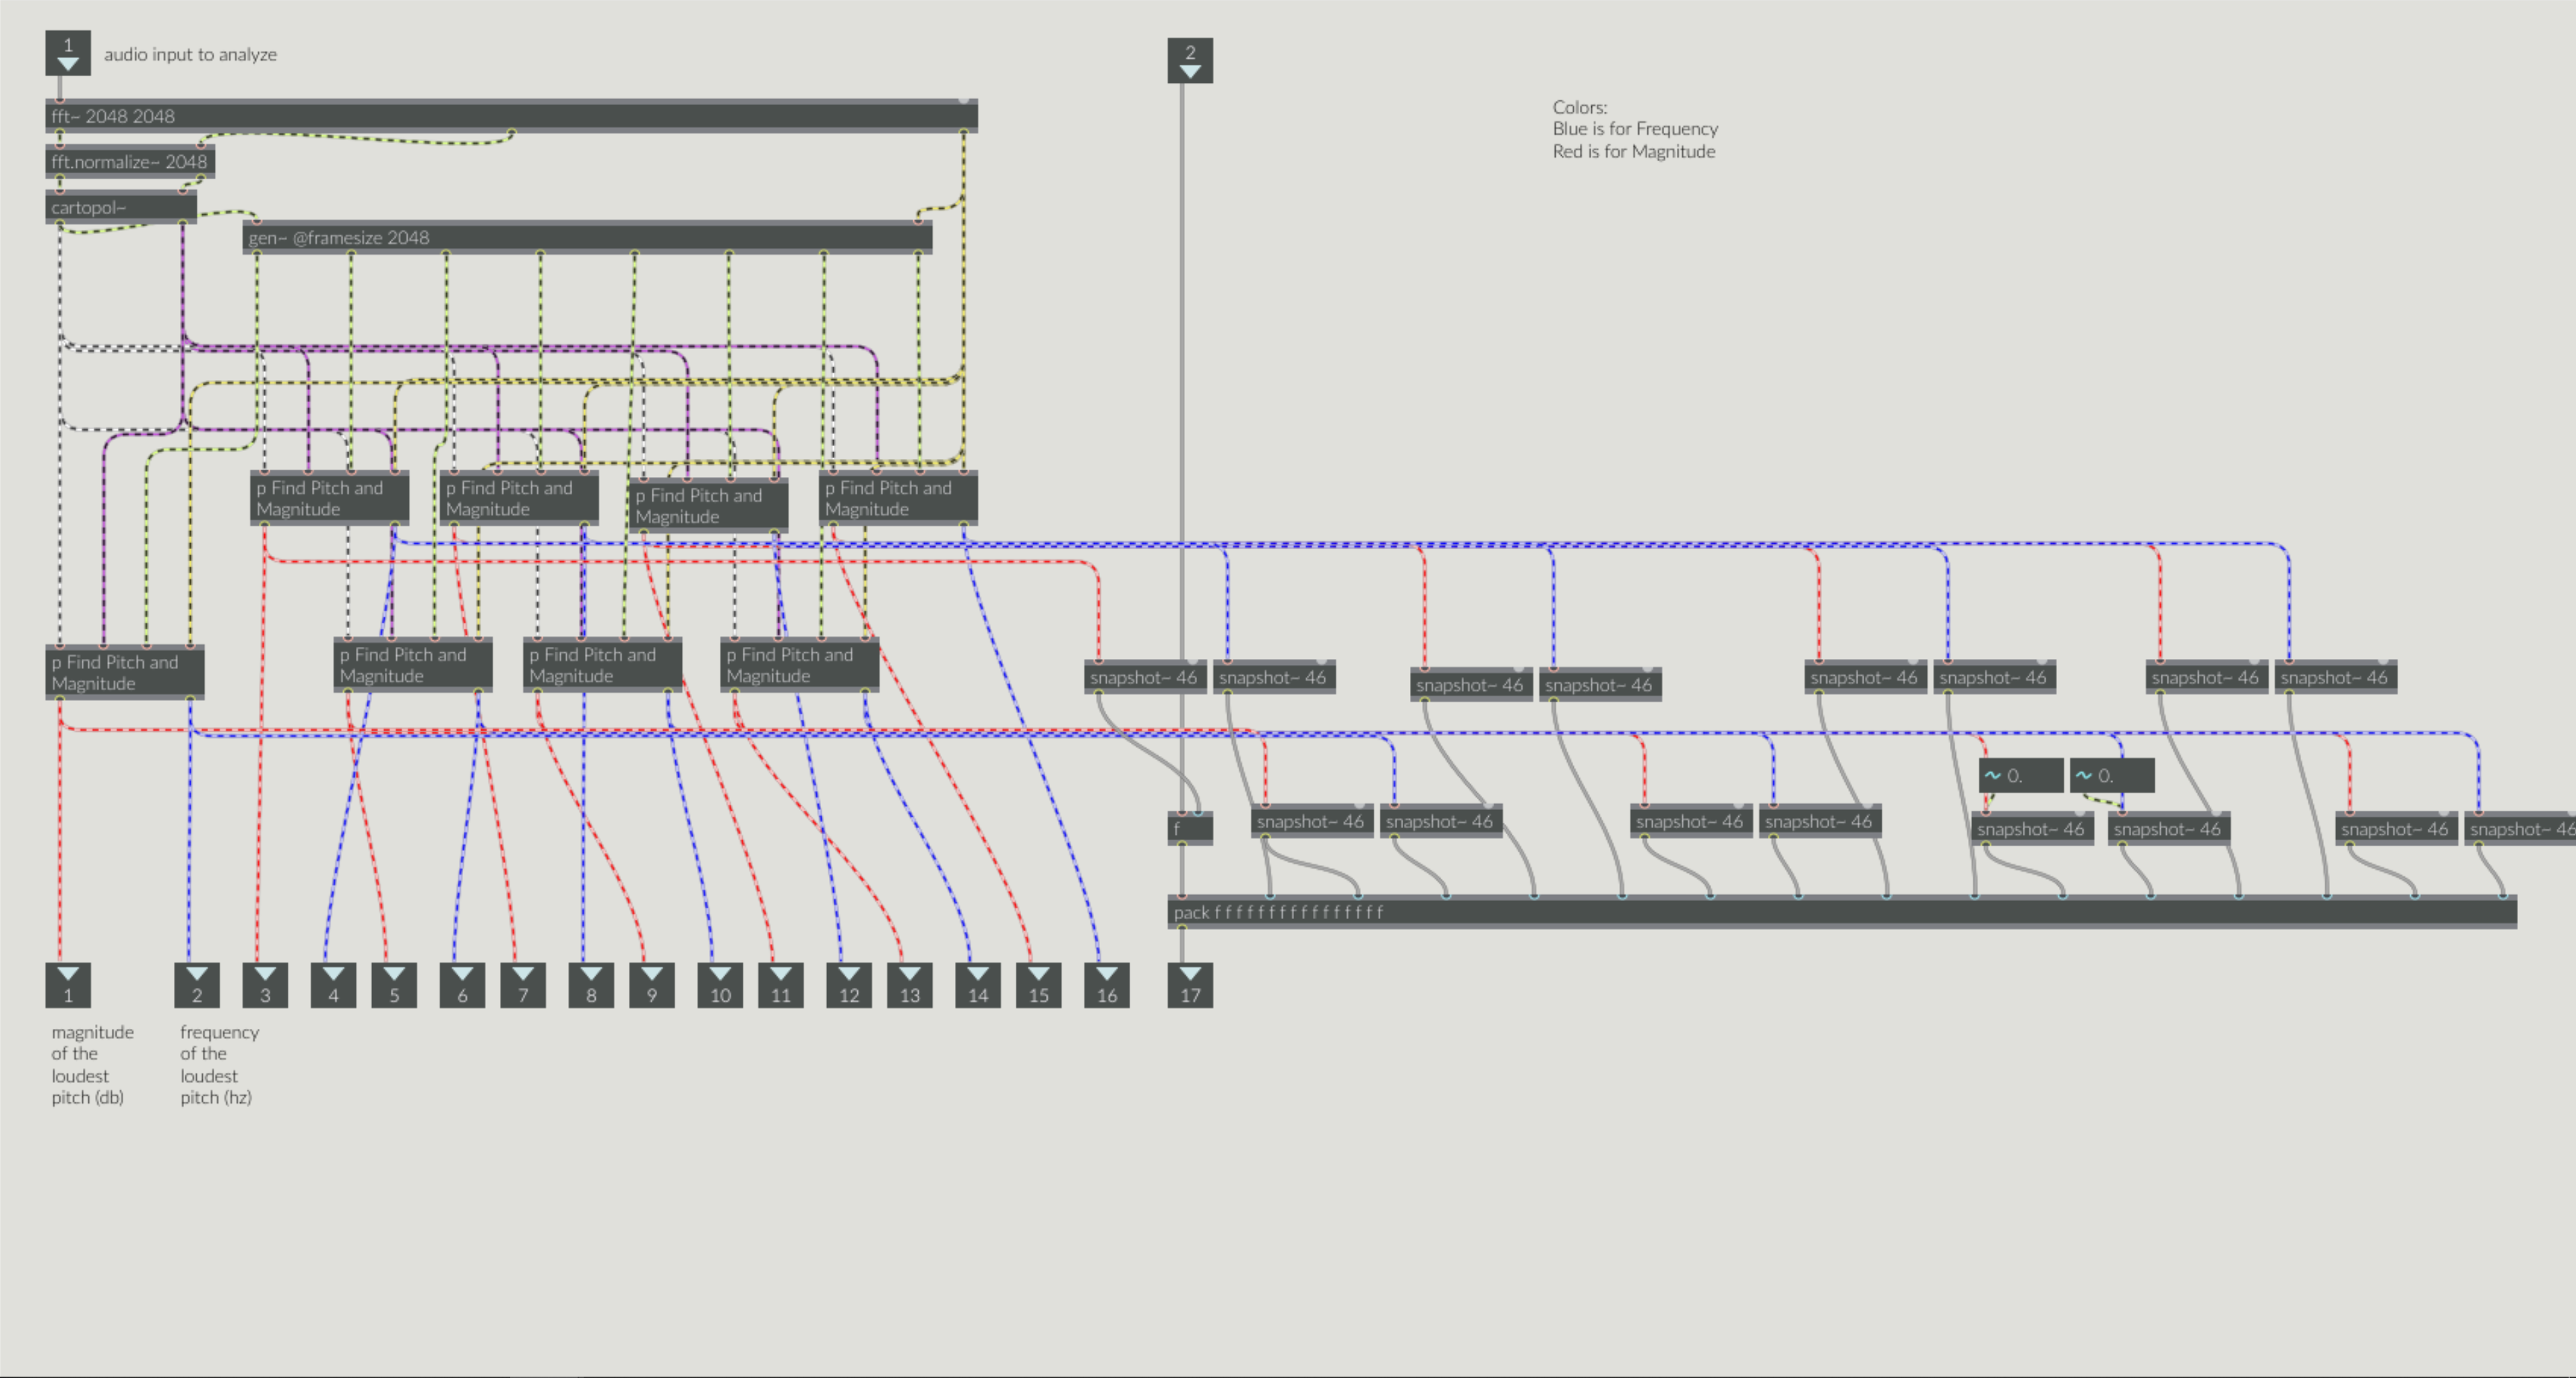
\includegraphics[width = \textwidth]{Graphs/MultipleTrack.png}
        \caption{Multiple Pitch tracking}
        \label{Analysis}
    \end{figure}

Afin de construire au mieux le patch, il est important de noter que la taille de la fenêtre affecte la qualité de la détection de la fréquence. La taille de la fenêtre influence la résolution temporelle ou fréquentielle de la représentation du signal. La résolution de fréquence peut être augmentée en modifiant la taille de la FFT, c'est-à-dire le nombre de segments de la fenêtre d'analyse. En particulier, la taille des bins correspond simplement à la moitié de la fenêtre d’analyse. La dispersion des fréquences est définie comme la division du SR par la taille de la fenêtre\footnote{Coralie Diatkine, \textit{AudioSculpt 3.0 User Manual}, 2011. \nocite{Audiosculpt}}.

    \begin{equation*}
        Frequency \; Range = \frac{SR}{Window \; Size}
    \end{equation*}

\section{Le vocodeur de phase}

Le vocodeur de phase est utilisé à l'origine pour la transposition de la hauteur et la modification de la vitesse de lecture. Pareillement, nous allons construire notre vocodeur de phase sur le modèle de base, puis nous proposerons quelques modifications. Le vocodeur de phase est étiqueté sous traitement spectral et va donc être stocké dans un objet \textit{pfft}$\thicksim $. Notre modèle est basé sur le vocodeur de phase par Dudas et Lippe\footnote{Richard Dudas et Cort Lippe, \textit{The Phase Vocoder}, 2006. \nocite{DL07} \nocite{DL06}}.

Pour accéder à un son directement dans l’objet \textit{pfft}$\thicksim$, il faut éviter d'utiliser les préréglages du  \textit{pfft}$\thicksim $. Par conséquent, nous allons éviter d'utiliser l'objet \textit{fftin}$ \thicksim $ à la place, nous allons utiliser un objet \textit{fft}$\thicksim $ dans un sous-patch. La seule différence est que les paramètres des objets \textit{fftin}$\thicksim $ et \textit{fftout}$\thicksim$ sont contrôlés directement à partir de l'objet  \textit{pfft}$\thicksim $ et que les entrées et sorties sont les premier et dernier objets. Pour construire un vocodeur de phase, nous devons traiter le son avant d'appliquer la transformation de Fourier. Pour comprendre la procédure on pourrait suivre le patch fourni dans la figure \ref{Phasevocoder}.

Le raisonnement derrière cette logique se repose sur le cœur du vocodeur de phase pour l'étirement sonore et le changement de la hauteur. Le vocodeur de phase nécessite une lecture indépendante du son à transformer pour chaque superposition de la FFT. Chaque image sonore de la lecture doit être synchronisée avec son image sonore respective de la FFT. Par conséquent, une seule copie du son ne peut pas être lancée dans un objet \textit{fftin}$\thicksim$, mais plutôt dans un objet \textit{fft}$\thicksim$. L'objet \textit{fft}$\thicksim$ exécute une FFT à spectre complet (c'est-à-dire en miroir), donc \textit{fft}$\thicksim$ peut fonctionner en synchronisation avec les images consécutives de la FFT traitées dans l'objet \textit{pfft}$\thicksim$ mais il est nécessaire de faire quelques modifications sur l'objet \textit{pfft}$\thicksim$ pour qu'il se comporte de la même manière.

Tout d'abord, l'objet \textit{pfft}$\thicksim$ doit traiter des images sonore de la FFT à spectre complet, au lieu de l'image spectrale par défaut qui correspond à la moitié de la taille de la FFT (jusqu'à la moitié de la fréquence de Nyquist). Cela peut être réalisé en ajoutant un cinquième argument non nul à l'objet \textit{pfft}$\thicksim$. Comme l'argument du spectre complet est le cinquième argument, nous devons fournir tous les autres arguments avant lui, y compris le quatrième argument (la position ou la FFT s’exécute) qui sera défini par défaut par zéro.

Ensuite, puisque les objets \textit{fftin}$\thicksim$ et \textit{fftout}$\thicksim$ effectuent le calcul de la FFT à la phase zéro par rapport à la FFT (le premier échantillon de la fenêtre envoyée au FFT est le milieu de la fenêtre), et les \textit{fft}$\thicksim$ et \textit{ifft}$\thicksim$ objets exécutent la FFT déphasée de 180 degrés, il faut assurer que tous les objets \textit{fftin}$\thicksim$ et \textit{fftout}$\thicksim$ du patch ont le même décalage de phase FFT utilisé dans les objets \textit{fft}$\thicksim$.

Cela peut être accomplie en spécifiant un déphasage par rapport aux objets \textit{fftin}$\thicksim$ et \textit{fftout}$\thicksim$. Une valeur de phase de $0.5$ signifie un déphasage de $180$ degrés, donc c'est la valeur préférable dans ce cas. Bien que, l'objet \textit{fftin}$\thicksim$ ne soit pas voulu, l'objet \textit{fftout}$\thicksim$ peut pratiquement être utilisé comme sortie pour l'objet \textit{pfft}$\thicksim$. Le fenêtrage automatique dans l'objet \textit{fftout}$\thicksim$ devrait se comporter comme le fenêtrage manuel avec les objets \textit{fft}$\thicksim$.

Dans cette version du vocodeur de phase, on va utiliser un son pré-déterminé. Cela veut dire qu'on utilisera un enregistrement et on le stockera dans un objet \textit{buffer}$\thicksim$. Le \textit{buffer}$\thicksim$ doit être accessible à deux endroits. Premièrement, à l'emplacement de l'image sonore de la FFT actuelle et, en deuxième lieu, à l'emplacement de l'image FFT précédente du \textit{buffer}$\thicksim$. Il est possible d'utiliser soit l'objet \textit{index}$\thicksim$ ou l'objet \textit{play}$\thicksim$\footnote{L'objet \textit{play}$\thicksim$ est utilisé comme interface de lecture de l'objet \textit{buffer}$\thicksim$. \textit{play}$\thicksim$ joue des samples en accord d'un offset parmi le buffer.} pour accéder au \textit{buffer}$\thicksim$. Lorsqu'on précise la position de la transformation Fourier en durée courte manuellement, on doit trouver un système pour préciser le décalage de la fenêtre dans notre \textit{buffer}$\thicksim$.

La solution dans cette problématique est d'utiliser deux objets \textit{fft}$\thicksim$ parallèles avec un décalage d'un quart, pour un chevauchement de $25 \%$. Un tel système permettra de calculer l'image actuelle de chaque index de la fenêtre en comparaison de l'index correspondant de la fenêtre précédente, comme cela a pu être fait dans le patch du pitch tracking. Le décalage est calculé pour une distance d'un quart puisqu'on prend en compte le paramètre du chevauchement. L'objet \textit{frameaccum}$\thicksim$ dans ce cas remplace la séquence des objets \textit{phasewrap}$\thicksim$, et normalisation entre $\pi$ et $-\pi$ qu'on a construit dans le patch du pitch tracking.

Pour la synchronisation du buffer on utilise un objet \textit{count}$\thicksim$ au paramètre $0$, la taille du fenêtrage, $1$ et $1$. On peut ainsi stocker la valeurs de l'échantillon exact au quelle la fenêtre de la FFT commence à la fois, ainsi que la position actuelle en durée totale du son. Chaque fois que le compteur se réinitialise à zéro, un objet \textit{sah}$\thicksim$ permet à la valeur de passer, dont on en déduit le premier sample de la FFT. En ajoutant les valeurs du compteur, on peut en déduire la position actuelle sur le fichier sonore. La valeur de la position sur le fichier nous permet de jouer le fichier à partir d'un objet \textit{play}$\thicksim$. 

On rappelle la formule du vocodeur de phase : 

    \begin{equation*}
    Phase \; Vocoder \; = \; \sum_{n=0} ^{N-1} h_a(n) \; x(n + uR_a) \; e^{-j \omega \frac{n}{N}} \vspace{0.5cm} 
    \end{equation*}
Dans la formule ci-dessus, on peut voir qu'il y a un fenêtrage correspondant, marqué $h_a(n)$. Pour simplifier, on va substituer avec quelques paramètres réels. On remplace $N$ par une taille de la fenêtre à $1024$ échantillons. On établit un décalage de 4 fois par fenêtre, donc $uR_a = (\frac{1}{4} * 1024)_a$ pour l'index $a$ de la fenêtre précédente.  
    \begin{equation*}
    Phase \; Vocoder \; = \; \sum_{n=0} ^{1023} h_a(n) \; x(n + 256_a) \; e^{-j \omega \frac{n}{1024}} \vspace{0.5cm} 
    \end{equation*}
À partir de cette formule, on peut identifier les éléments qui la reproduise dans le patch Max. La fonction, correspondant à la phase de l'analyse, contient la somme des échantillons du signal qui appartiennent à la taille de la fenêtre de la FFT, plus des échantillons qui appartiennent $\Sigma_n (x_n) $ à la fenêtre décalée par la taille du \textit{hop}, $uR_a$. Les échantillons sont multipliées, par une fenêtrage $h_a(n)$ et ensuite par la formule d'Euler qui équivaut à la transformation de Fourier.

    \begin{figure}
        \centering
        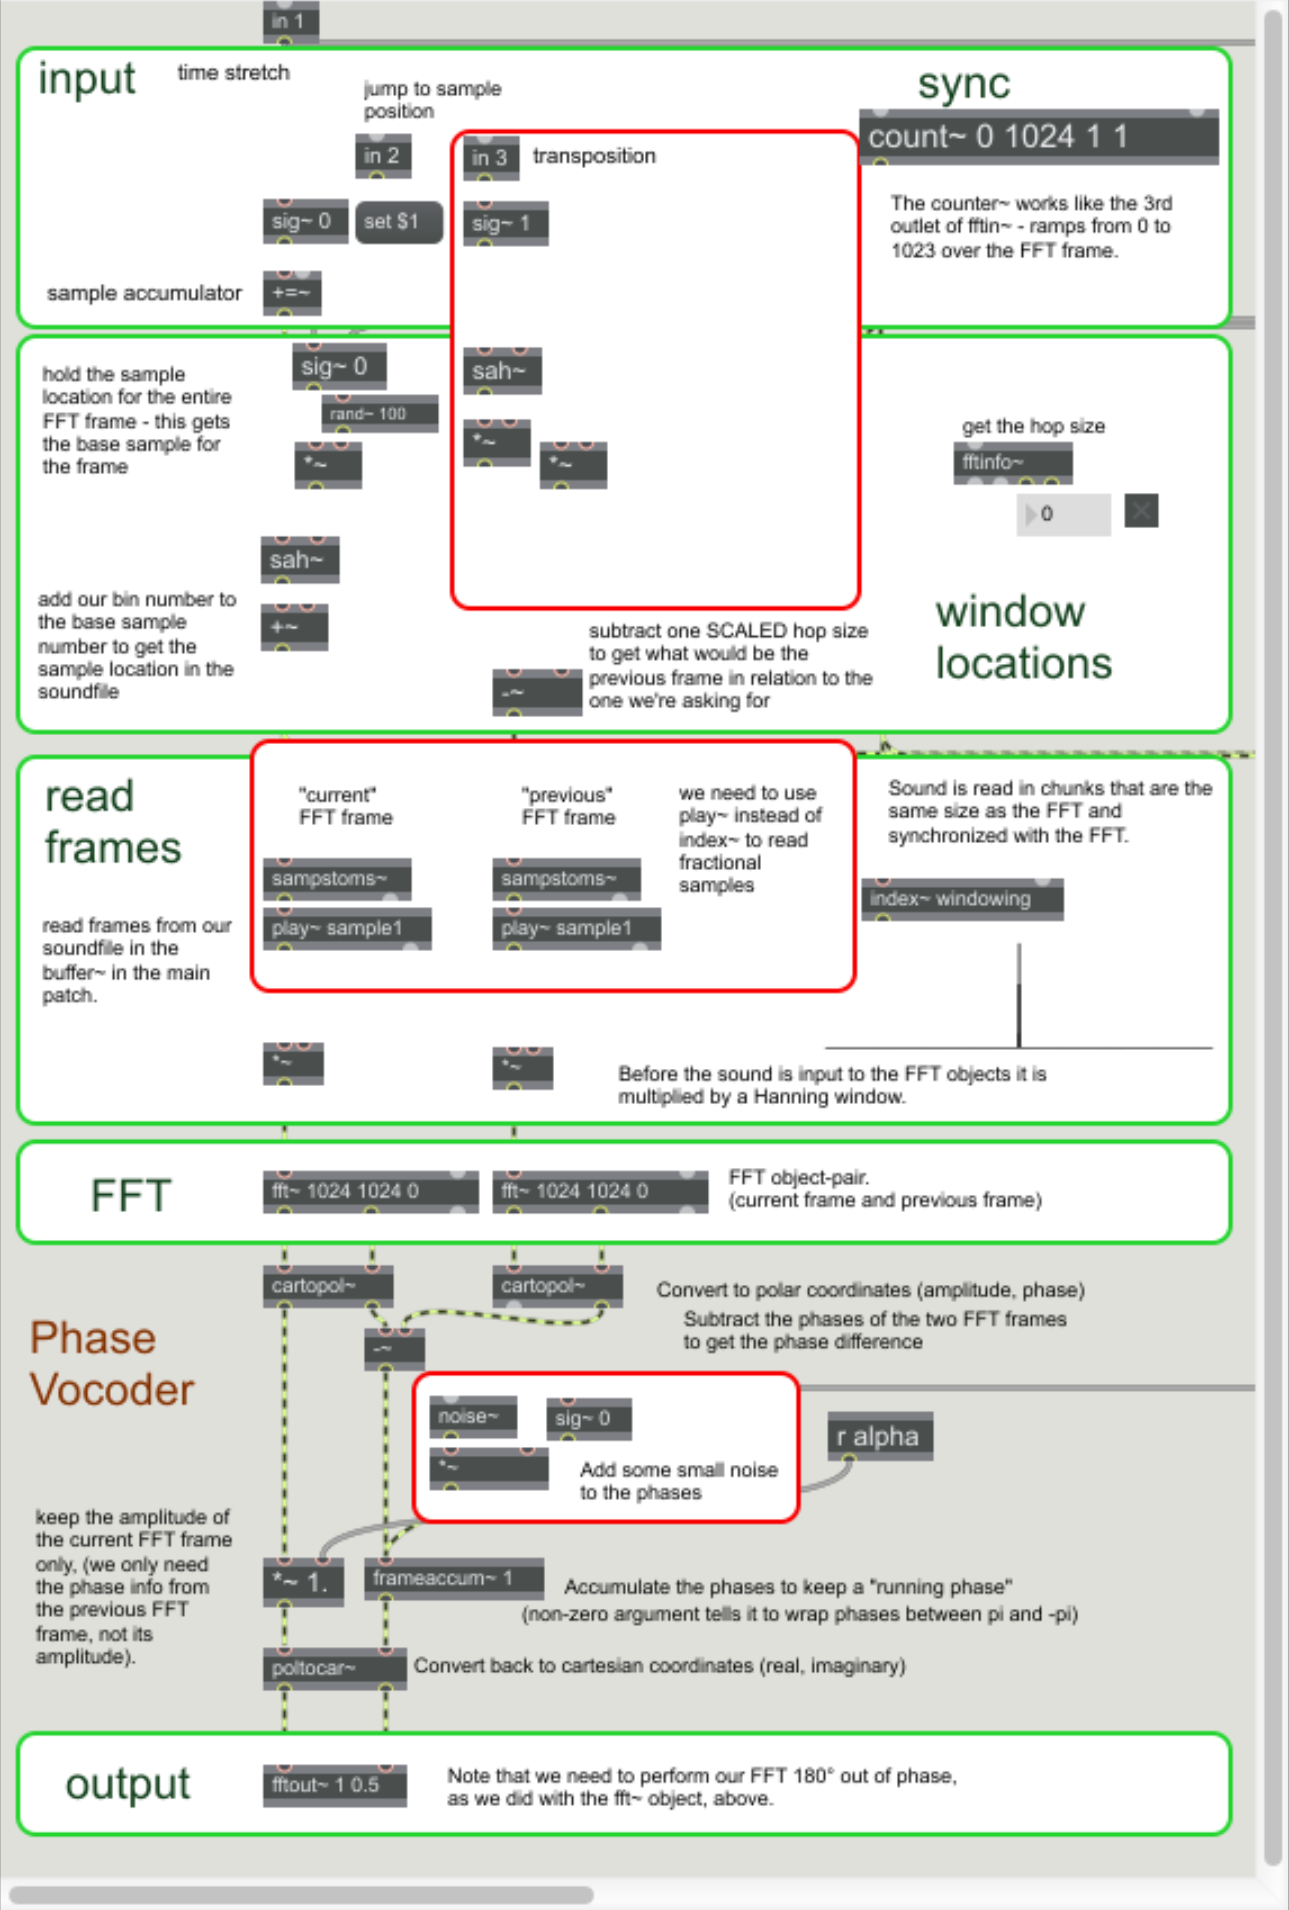
\includegraphics[width = \textwidth]{Graphs/PhaseVocoder.png}
        \caption{Le vocodeur de phase}
        \label{Phasevocoder}
    \end{figure}
    
Nous pouvons voir qu'une fonctionnalité de fenêtrage est inclu à la fois dans la formule et dans le patch présenté. Au lieu d'utiliser une fenêtre par défaut de l'objet \textit{fft}$\thicksim $, nous allons utiliser un buffer fixé de taille $ N $. En utilisant l'objet \textit{count}$\thicksim $ avec l'aide de l'objet \textit{index}$\thicksim$ \footnote{L'objet \textit{index}$\thicksim $ est utilisé pour lire un objet $ buffer \thicksim $ dans un exemple d'index piloté par signal sans interpolation sur la sortie.}, pour accéder à chaque échantillon, on multiplie le son de l'entre par les valeurs du fenêtrage avant d'effectuer de la FFT.

\subsubsection{Filtre Gabor}

Dans la section 2, nous avons présenté le filtrage de Gabor. Dans cette section, nous allons créer un filtre Gabor personnalisé. La formule de Gabor normalisée permet de modifier la courbe de la fonction gaussienne tout en conservant les constantes de valeurs maximales et minimales. Cette fenêtre gaussienne faite sur mesure est présentée en figure \ref{windowing}.

Nous utilisons un objet \textit{uzi}\footnote{Envoyer instantanément le nombre de \guillemotleft bangs \guillemotright qui ont été définies dans la position de l'argument de l'objet.} avec argument la taille de la fenêtre FFT, suivie de l'expression effectuant une courbe gaussienne normalisée. Ensuite, nous l'envoyons dans le buffer nommé \guillemotleft windowing \guillemotright à l'aide de l'objet \textit{peek}$ \thicksim $ \footnote{L'objet \textit{peek}$ \thicksim $ est utilisé pour lire et écrire des de valeurs des échantillons dans un \textit{buffer}$ \thicksim $ }. Bien sûr, dans ce cas, le filtre de Gabor n’est pas directement exécuté pendant la FFT, mais juste avant. En utilisant ce filtrage, nous pouvons librement chevaucher des fenêtres et éviter des artefacts.
    
    \begin{figure}
        \centering
        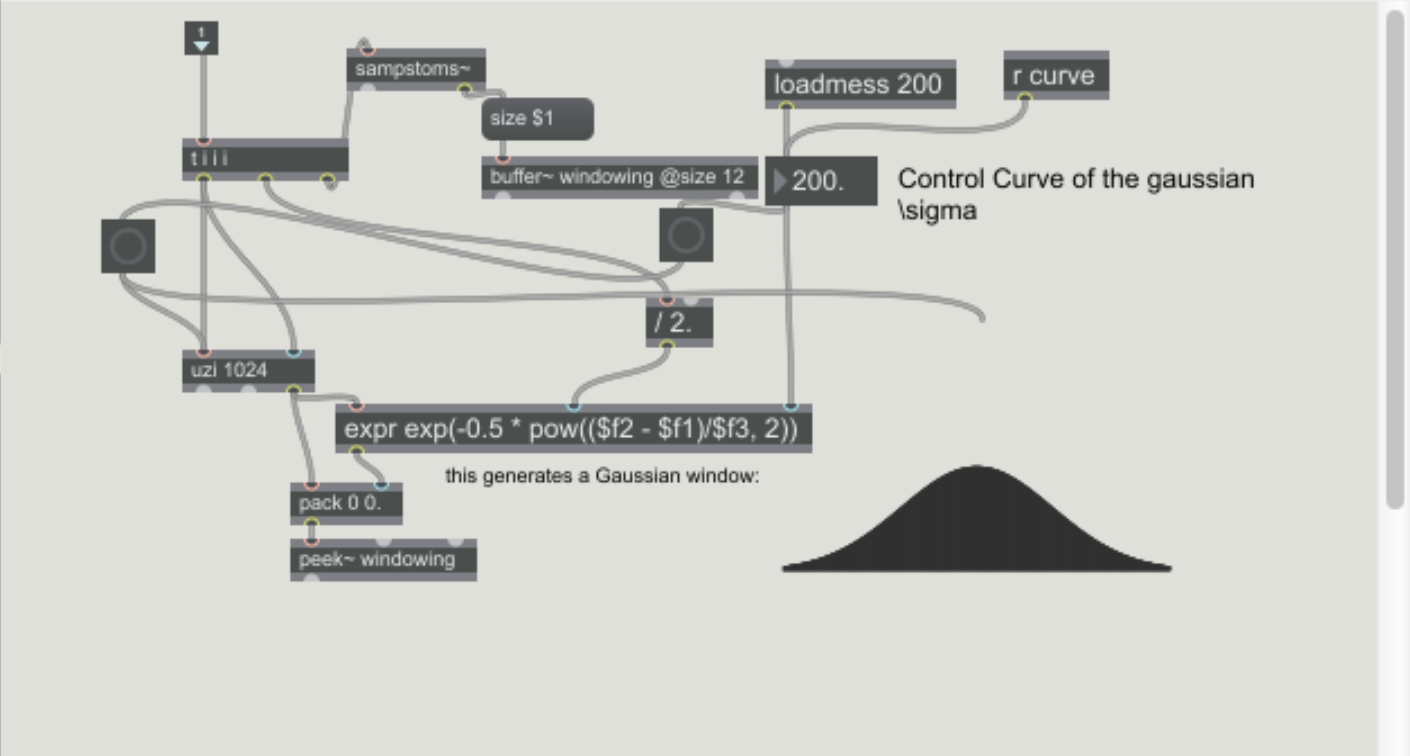
\includegraphics[width = \textwidth]{Graphs/windowing.png}
        \caption{Fenêtrage gaussien}
        \label{windowing}
    \end{figure}

\subsubsection{Transposition de la hauteur}

    Pour appliquer la transposition de la hauteur avec le vocodeur de phase, il convient de modifier le facteur de la hauteur tout en modifiant simultanément la fréquence d'échantillonnage. Par exemple, afin de transposer un son d'une octave plus basse, nous devons reproduire le son à une vitesse deux fois moins rapide, tout en doublant le SR. En utilisant cette méthode, il est possible de changer la hauteur en modifiant la vitesse de lecture.

    Pour utiliser cette méthode, nous utilisons des valeurs MIDI standard traduites en fréquence et adaptées au chevauchement des fenêtres. L'utilisateur peut ensuite saisir la valeur dans un piano midi virtuel, facilitant ainsi la manipulation. Par défaut, la note midi Do avec la valeur 60 est la hauteur standard. Ensuite, la hauteur change en fonction de l'intervalle en fonction de la valeur par défaut. Par conséquent, la valeur Do une octave inférieure dans le piano midi virtuel correspond à une octave de transposition inférieure à la hauteur originale du son.

    À l'intérieur du vocodeur de phase, le décalage de hauteur est traduit par le saut d'échantillons ou le sur-échantillonnage de l'objet  \textit{count}$\thicksim $. Bien sûr, augmenter le SR n'est pas une solution valable, nous avons donc choisi de prendre une portion plus petite ou plus grande du \textit{buffer}$\thicksim $ correspondant à la taille de la fenêtre. Une transposition vers le haut correspond au fait de prendre une fenêtre plus grande dans \textit{buffer}$\thicksim $ et de la lire à une vitesse plus rapide, tandis qu'un décalage de hauteur correspond à couper une plus petite partie de la variable \textit{buffer}$\thicksim $ et à la lire plus lentement.

    Pour cet exemple, nous utilisons un objet \textit{sah}$\thicksim $ pour nous assurer que la valeur de transposition est maintenue constante pour tous les bins pendant la FFT. Ensuite, nous multiplions par la valeur actuelle du compteur et nous ajoutons la valeur de sortie au nombre d'échantillons déjà lus pour obtenir l'emplacement souhaité du fichier. En ce qui concerne la fréquence initiale $ \omega $, le décalage individuel s’élève à:

    \begin{equation*}
        \Delta \omega(\omega) = \omega (\alpha - 1)
    \end{equation*}

    Où $ \alpha $ est le facteur de transposition et $ \Delta \omega $ la différence de fréquence. Cette technique impose une transposition de fréquence constante $ \Delta \omega $ à toutes les fréquences détectées de la FFT.

    L'implémentation Pitch Shifting peut être vue dans la figure. Quelques objets suffisent pour implémenter un décalage de hauteur sur le corps de base du vocodeur de phase.


\subsubsection{Modulation Temporelle}

    Comme il a été étudié à la section 2, modifier la vitesse de lecture tout en gardant la hauteur du pitch stable est l’opération inverse de la transposition de la hauteur. La lecture peut être contrôlée en prenant en compte le facteur de chevauchement des fenêtres FFT. On peut diviser par le facteur du chevauchement et ajouter le pourcentage de la lecture souhaitée. À l'intérieur du vocodeur, la valeur factorisée est ajoutée à l'accumulateur d'échantillons. Dans ce cas, la valeur de la vitesse de lecture est ajoutée sur la position de l'interprétation de chaque échantillon. Une lecture plus rapide peut enjamber des échantillons où une vitesse de lecture plus lente lit plusieurs fois chaque échantillon. La soustraction de la position précédente de chaque échantillon (la fenêtre de la FFT), fixe les déviations de fréquence. 

\section{Morphing spectrale}

La démonstration finale de ce chapitre est une implémentation du morphing spectral ou de la synthèse croisée spectrale. Pour accomplir cette technique, nous utilisons deux vocodeurs en phase parallèles et nous interpolons la phase et l’amplitude entre toute indice du bin. Pour comprendre la complexité computationnelle du morphing spectral, rappelons-nous qu'un vocodeur à phase simple utilise deux FFT parallèles décalées du facteur de fenêtre de recouvrement. Donc, si nous utilisons une fenêtre de 1024 échantillons et un facteur de chevauchement de 4, la première FFT commence en position $ 0 $ et la fenêtre parallèle en position d’échantillon $256$. Nous utilisons maintenant 4 FFT parallèles pour le morphing spectral. Cela fait une prix computationnelle relativement haute, mais il reste possible de le calculer avec les ordinateurs actuels.

Dans ce double vocodeur de phase, les sorties de l'objet \textit{cartopol}$ \thicksim $, la magnitude et la phase après l'analyse de Fourier, sont multipliées par le facteur d'interpolation de morphing. La phase est préalablement corrigée par une accumulation avec l'harmonique précédente et une petite quantité de bruit est ajoutée pour la naturalisation du résultât sonore. Nous séparons les canaux d’interpolation de magnitude et de phase. Ainsi, on peut préférer émettre, par exemple, l’amplitude du son source mais la phase du son cible.

La sortie de chaque son après l’interpolation est transformée en forme cartésienne et une FFT inverse est appliquée. Ainsi, nous obtenons un résultat sonore homogène. À ce stade, un certain nombre d'opérations d'édition peuvent être ajoutées, telles que la modélisation du bruit ou une interpolation variable par image, etc. Mais avant de plonger dans des modifications avancées, examinons d'abord les techniques d'interpolation.

L'interpolation est définie par défaut sur linéaire. Un simple code Javascript que nous avons implémenté crée une courbe linéaire. Les valeurs d'interpolation varient entre $ [0, 1] $. La valeur $ 0 $ correspond à une interpolation nulle, et par conséquent la magnitude ou la phase du son source est sortie. Une valeur de $ 1 $ restitue entièrement les caractéristiques du son target et omet le son source. Une courbe linéaire définit une méthode linéaire pour interpoler les sons. En allons plus loin, nous implémentons un certain nombre de courbes telles que exponentielle, logarithmique et, bien entendu, linéaire. Par conséquent, il existe différentes manières d'interpoler des sons en fonction de leurs composantes de fréquence ou de la magnitude de leurs composantes de fréquence. Toutes les interpolations varient entre la même intégrale $ [0, 1] $. Le code Javascript peut être consulté dans le bout de code ci-dessous.

La version du vocodeur de phase pour le morphing spectral est montrée dans la figure \ref{Morphing}. Il existe deux buffers, un pour la source et un pour le son target. Le fenêtrage gaussien pour du filtrage Gabor, avec une courbe normalisée à distance, est aussi paramétrable dans la plateforme. Un bouton d’interpolation pour la phase et un bouton pour l’interpolation de la magnitude contrôlent les facteurs d’interpolation pour le morphing et une factorisation du bruit pour la naturalisation de la phase sont mis en œuvre.

    \begin{figure}
        \centering
        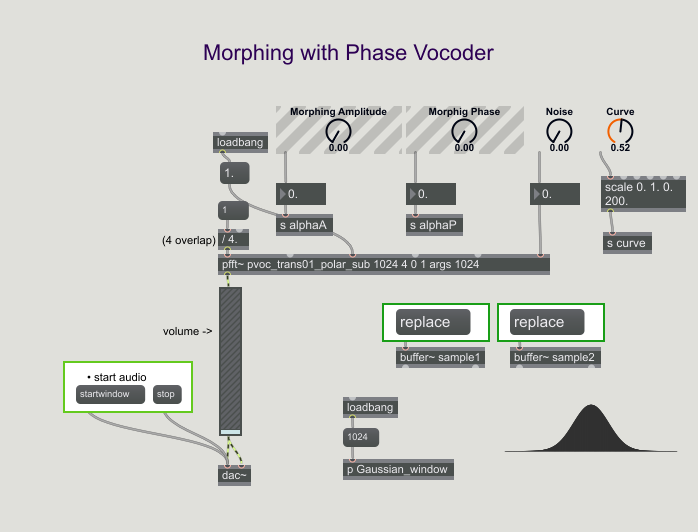
\includegraphics[width = \textwidth]{Graphs/SoundMorphing.png}
        \caption{Morphing en temps réel}
        \label{Morphing}
    \end{figure}


\noindent\begin{minipage}{\textwidth}
\lstinputlisting[language=Java]{Expondential.js}
\end{minipage}